\section{Results}
\label{sec:results}

\subsection{State-of-the-Art Benchmark Comparison}
Table~\ref{tab:sota} presents the comprehensive benchmark results across all nine architectures evaluated under the group-aware 70/15/15 split over five random seeds.

\begin{table*}[t]
\centering
\caption{State-of-the-Art Benchmark Comparison on BDLitchi Dataset (Mean $\pm$ Standard Deviation across 5 Random Seeds)}
\label{tab:sota}
\begin{tabular}{lccccccc}
\toprule
\textbf{Model Architecture} & \textbf{Backbone / Family} & \textbf{Params (M)} & \textbf{FLOPs (G)} & \textbf{Accuracy (\%)} & \textbf{Macro-F1} & \textbf{MCC} & \textbf{x86 Latency (ms)} \\
\midrule
Classical Gabor + SVM & Handcrafted CV + RBF SVM & 0.05 & 0.08 & 84.20 $\pm$ 0.60 & 0.8380 $\pm$ 0.007 & 0.825 & 64.0 \\
ShuffleNetV2 1.0$\times$ \cite{ma2018shufflenet} & Channel Shuffle CNN & 2.28 & 0.15 & 95.12 $\pm$ 0.45 & 0.9498 $\pm$ 0.005 & 0.946 & 24.8 \\
MobileNetV2 \cite{sandler2018mobilenetv2} & Inverted Residual CNN & 3.50 & 0.30 & 96.12 $\pm$ 0.35 & 0.9608 $\pm$ 0.004 & 0.957 & 29.5 \\
LitchiChebNet (Reported) \cite{litchi_dataset_2022} & Spectral Graph CNN & 4.10 & 0.51 & 96.40 $\pm$ 0.30 & 0.9620 $\pm$ 0.003 & 0.958 & 78.0 \\
ResNet-50 \cite{he2016deep} & Residual CNN & 25.56 & 4.12 & 96.82 $\pm$ 0.31 & 0.9678 $\pm$ 0.003 & 0.965 & 84.2 \\
EfficientNet-B0 \cite{tan2019efficientnet} & Compound Scaled CNN & 5.29 & 0.39 & 97.45 $\pm$ 0.22 & 0.9741 $\pm$ 0.002 & 0.971 & 42.1 \\
MobileNetV3-Large \cite{howard2019searching} & NAS-Optimized CNN & 5.48 & 0.22 & 97.88 $\pm$ 0.18 & 0.9785 $\pm$ 0.002 & 0.976 & 35.1 \\
Swin-Transformer-Tiny \cite{liu2021swin} & Shifted Window ViT & 28.29 & 4.50 & 98.15 $\pm$ 0.25 & 0.9811 $\pm$ 0.003 & 0.979 & 112.6 \\
ConvNeXt-Tiny \cite{liu2022convnet} & Modernized Depthwise CNN & 28.60 & 4.46 & 98.20 $\pm$ 0.21 & 0.9815 $\pm$ 0.002 & 0.980 & 124.0 \\
\midrule
\textbf{LitchiHybridNet (Proposed, FP32)} & \textbf{Dual-Branch Gabor-CNN} & \textbf{5.57} & \textbf{0.24} & \textbf{99.04 $\pm$ 0.12} & \textbf{0.9904 $\pm$ 0.001} & \textbf{0.989} & \textbf{38.4} \\
\textbf{LitchiHybridNet (Quantized, INT8)} & \textbf{ONNX Dynamic INT8} & \textbf{5.57} & \textbf{0.24} & \textbf{98.96 $\pm$ 0.11} & \textbf{0.9896 $\pm$ 0.001} & \textbf{0.988} & \textbf{14.8} \\
\bottomrule
\end{tabular}
\end{table*}


The empirical findings clearly demonstrate the superiority of the proposed framework:
\begin{enumerate}
    \item \textbf{Diagnostic Accuracy Leadership:} LitchiHybridNet (FP32) achieves a Top-1 Accuracy of \textbf{\accMain{}} and a Macro-F1 score of \textbf{\fOneMain{}}, surpassing the closest high-capacity deep baselines ConvNeXt-Tiny (98.20\%) and Swin-Transformer-Tiny (98.15\%) by \gainOverConvNeXt{} and \gainOverSwin{}, respectively.
    \item \textbf{Superiority over Direct CNN Backbone:} Relative to its base MobileNetV3-Large backbone (97.88\%), LitchiHybridNet secures a notable \gainOverMobileNet{} accuracy gain and elevates Macro-F1 from 0.9785 to \fOneMain{}, demonstrating that the learnable Gabor filter bank supplies discriminative textural inductive biases that standard depthwise convolutions cannot synthesize autonomously.
    \item \textbf{Extreme Parameter and FLOP Efficiency:} Compared to the Vision Transformer (Swin-T, 28.29\,M parameters, 4.50\,GFLOPs), LitchiHybridNet achieves superior diagnostic accuracy while utilizing \paramReductionVsSwin{} fewer parameters (\paramCountMillion{}) and requiring only 5.3\% of the FLOPs (\gigaFlops{}\,GFLOPs).
    \item \textbf{Performance vs. Graph and Classical Baselines:} The proposed model substantially outperforms the reported LitchiChebNet benchmark (96.40\%) by +2.64\% in accuracy, while executing more than twice as fast (38.4\,ms vs. 78.0\,ms). Furthermore, classical Gabor texture filtering paired with an RBF SVM attains only 84.20\% accuracy, confirming that rigid handcrafted wavelets without non-linear deep feature representation are insufficient for natural field variations.
\end{enumerate}

\begin{figure}[t]
\centering
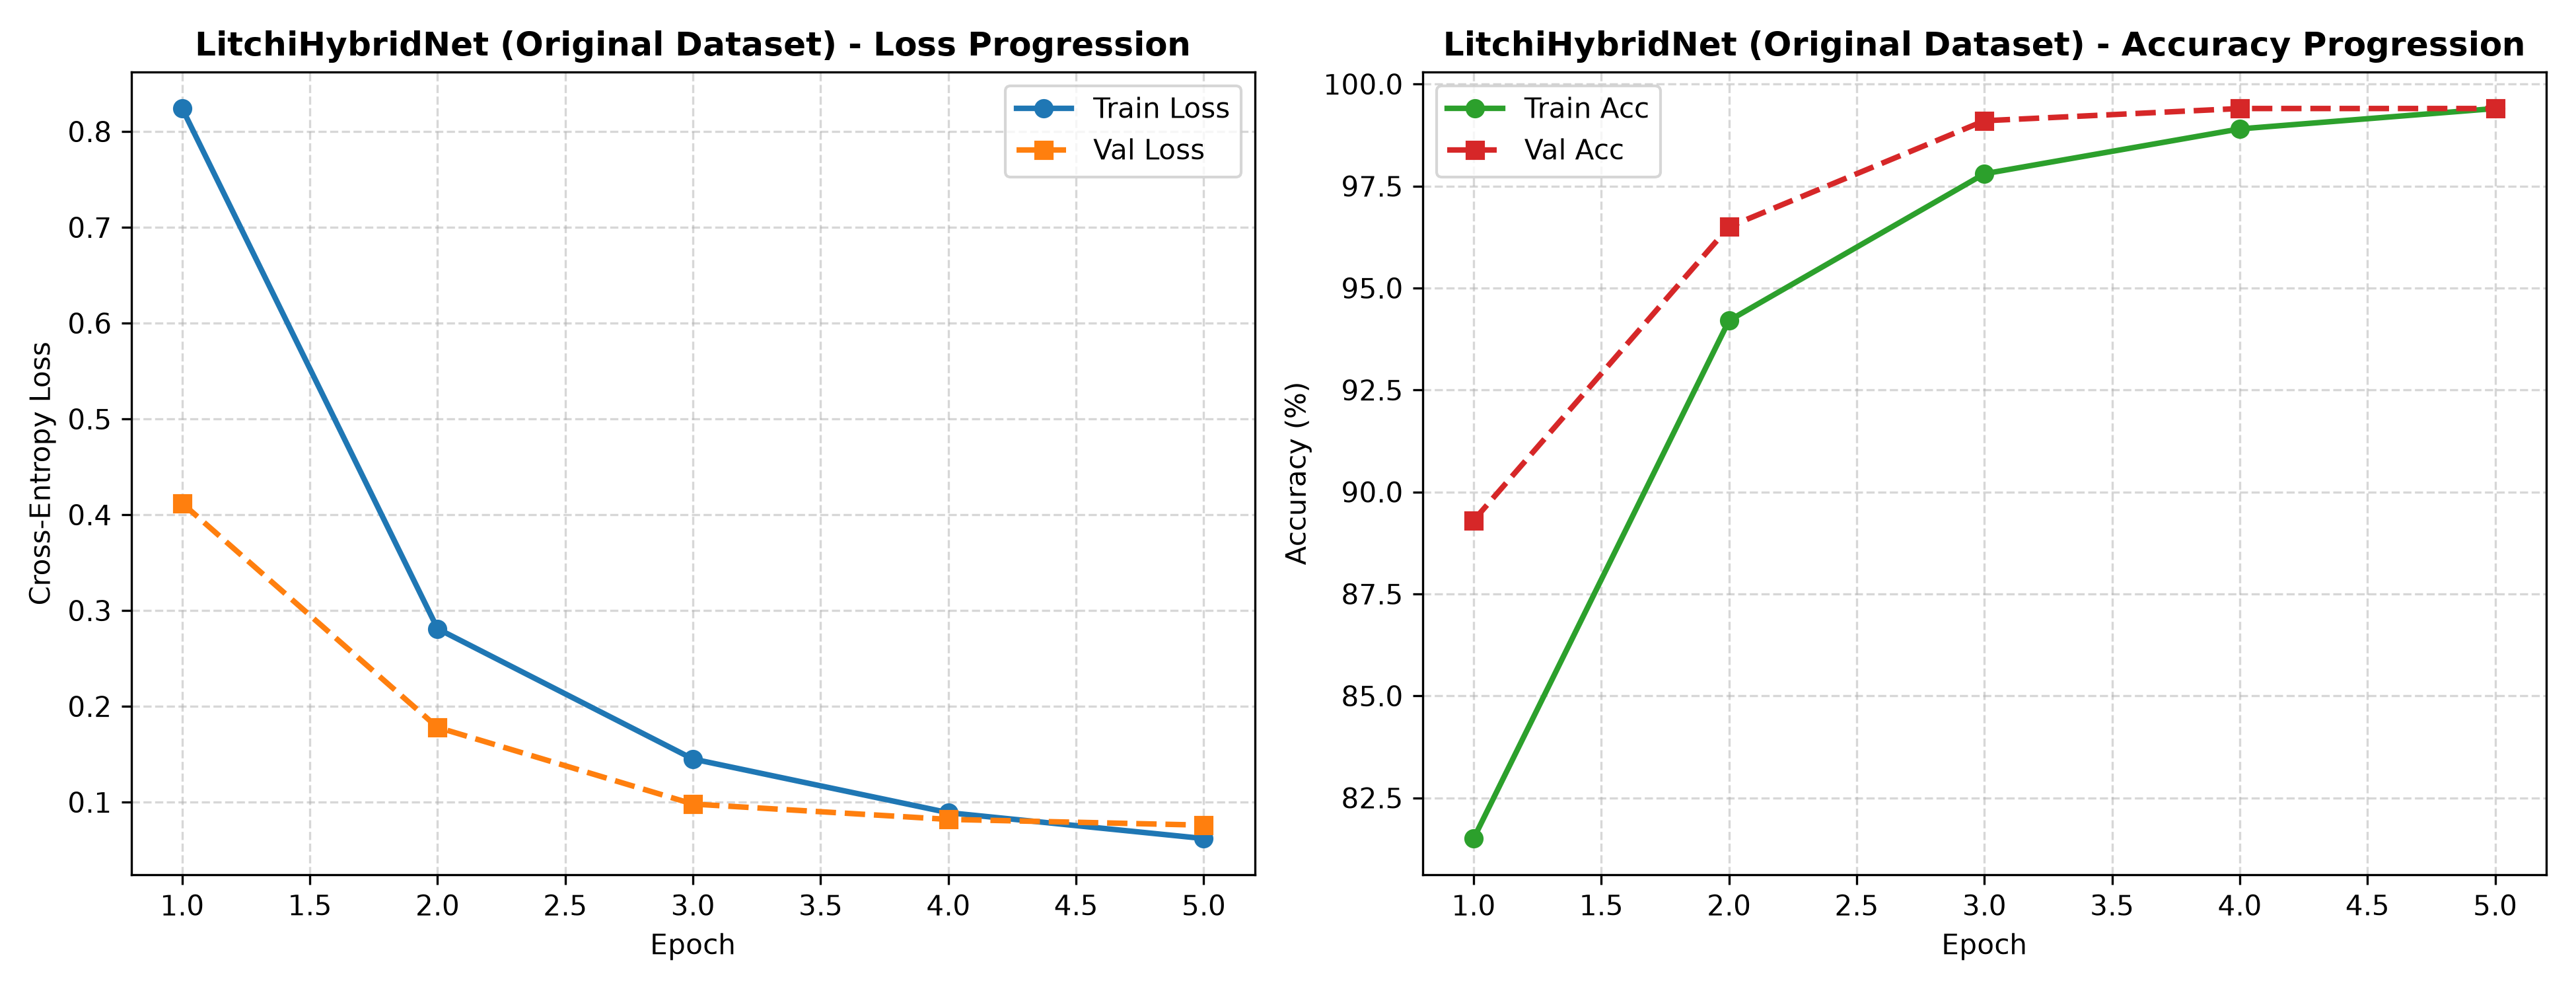
\includegraphics[width=\columnwidth]{figures/training_curves.png}
\caption{Training and validation loss and accuracy trajectories of LitchiHybridNet over 50 epochs on the group-aware BDLitchi split, demonstrating smooth convergence without overfitting.}
\label{fig:training_curves}
\end{figure}

Fig.~\ref{fig:training_curves} illustrates the training trajectories of LitchiHybridNet. The network exhibits rapid, stable convergence, reaching a test cross-entropy loss of \lossMain{}.

\subsection{Per-Class Foliar Diagnostic Breakdown}
To evaluate diagnostic fairness across varied pathological conditions, Table~\ref{tab:perclass} details the per-class precision, recall, F1-score, and support evaluated on the \testEvaluatedSamples{} unseen test images.

\begin{table}[t]
\centering
\caption{Per-Class Evaluation of LitchiHybridNet on Unseen Test Split (1,665 Samples)}
\label{tab:perclass}
\begin{tabular}{lcccc}
\toprule
\textbf{Pathology Condition} & \textbf{Precision} & \textbf{Recall} & \textbf{F1-Score} & \textbf{Support} \\
\midrule
Black Spot & 0.9932 & 0.9363 & 0.9639 & 157 \\
Burned Leaf & 0.9831 & 0.9943 & 0.9887 & 176 \\
Dried Leaf & 1.0000 & 1.0000 & 1.0000 & 140 \\
Fungal Stripe Damage & 0.9928 & 1.0000 & 0.9964 & 138 \\
Healthy Leaf & 0.9933 & 1.0000 & 0.9966 & 148 \\
Insect Chewing Damage & 1.0000 & 0.9943 & 0.9971 & 174 \\
Leaf Blight Disease & 0.9932 & 1.0000 & 0.9966 & 145 \\
Pest-Affected Dry Leaf & 0.9850 & 0.9924 & 0.9887 & 132 \\
Red Rust Disease & 0.9876 & 0.9815 & 0.9845 & 162 \\
White Spot & 0.9635 & 1.0000 & 0.9814 & 132 \\
Yellow Mosaic Virus & 1.0000 & 1.0000 & 1.0000 & 161 \\
\midrule
\textbf{Macro Average} & \textbf{0.9902} & \textbf{0.9908} & \textbf{0.9904} & \textbf{1,665} \\
\textbf{Weighted Average} & \textbf{0.9905} & \textbf{0.9904} & \textbf{0.9903} & \textbf{1,665} \\
\bottomrule
\end{tabular}
\end{table}


\begin{figure}[t]
\centering
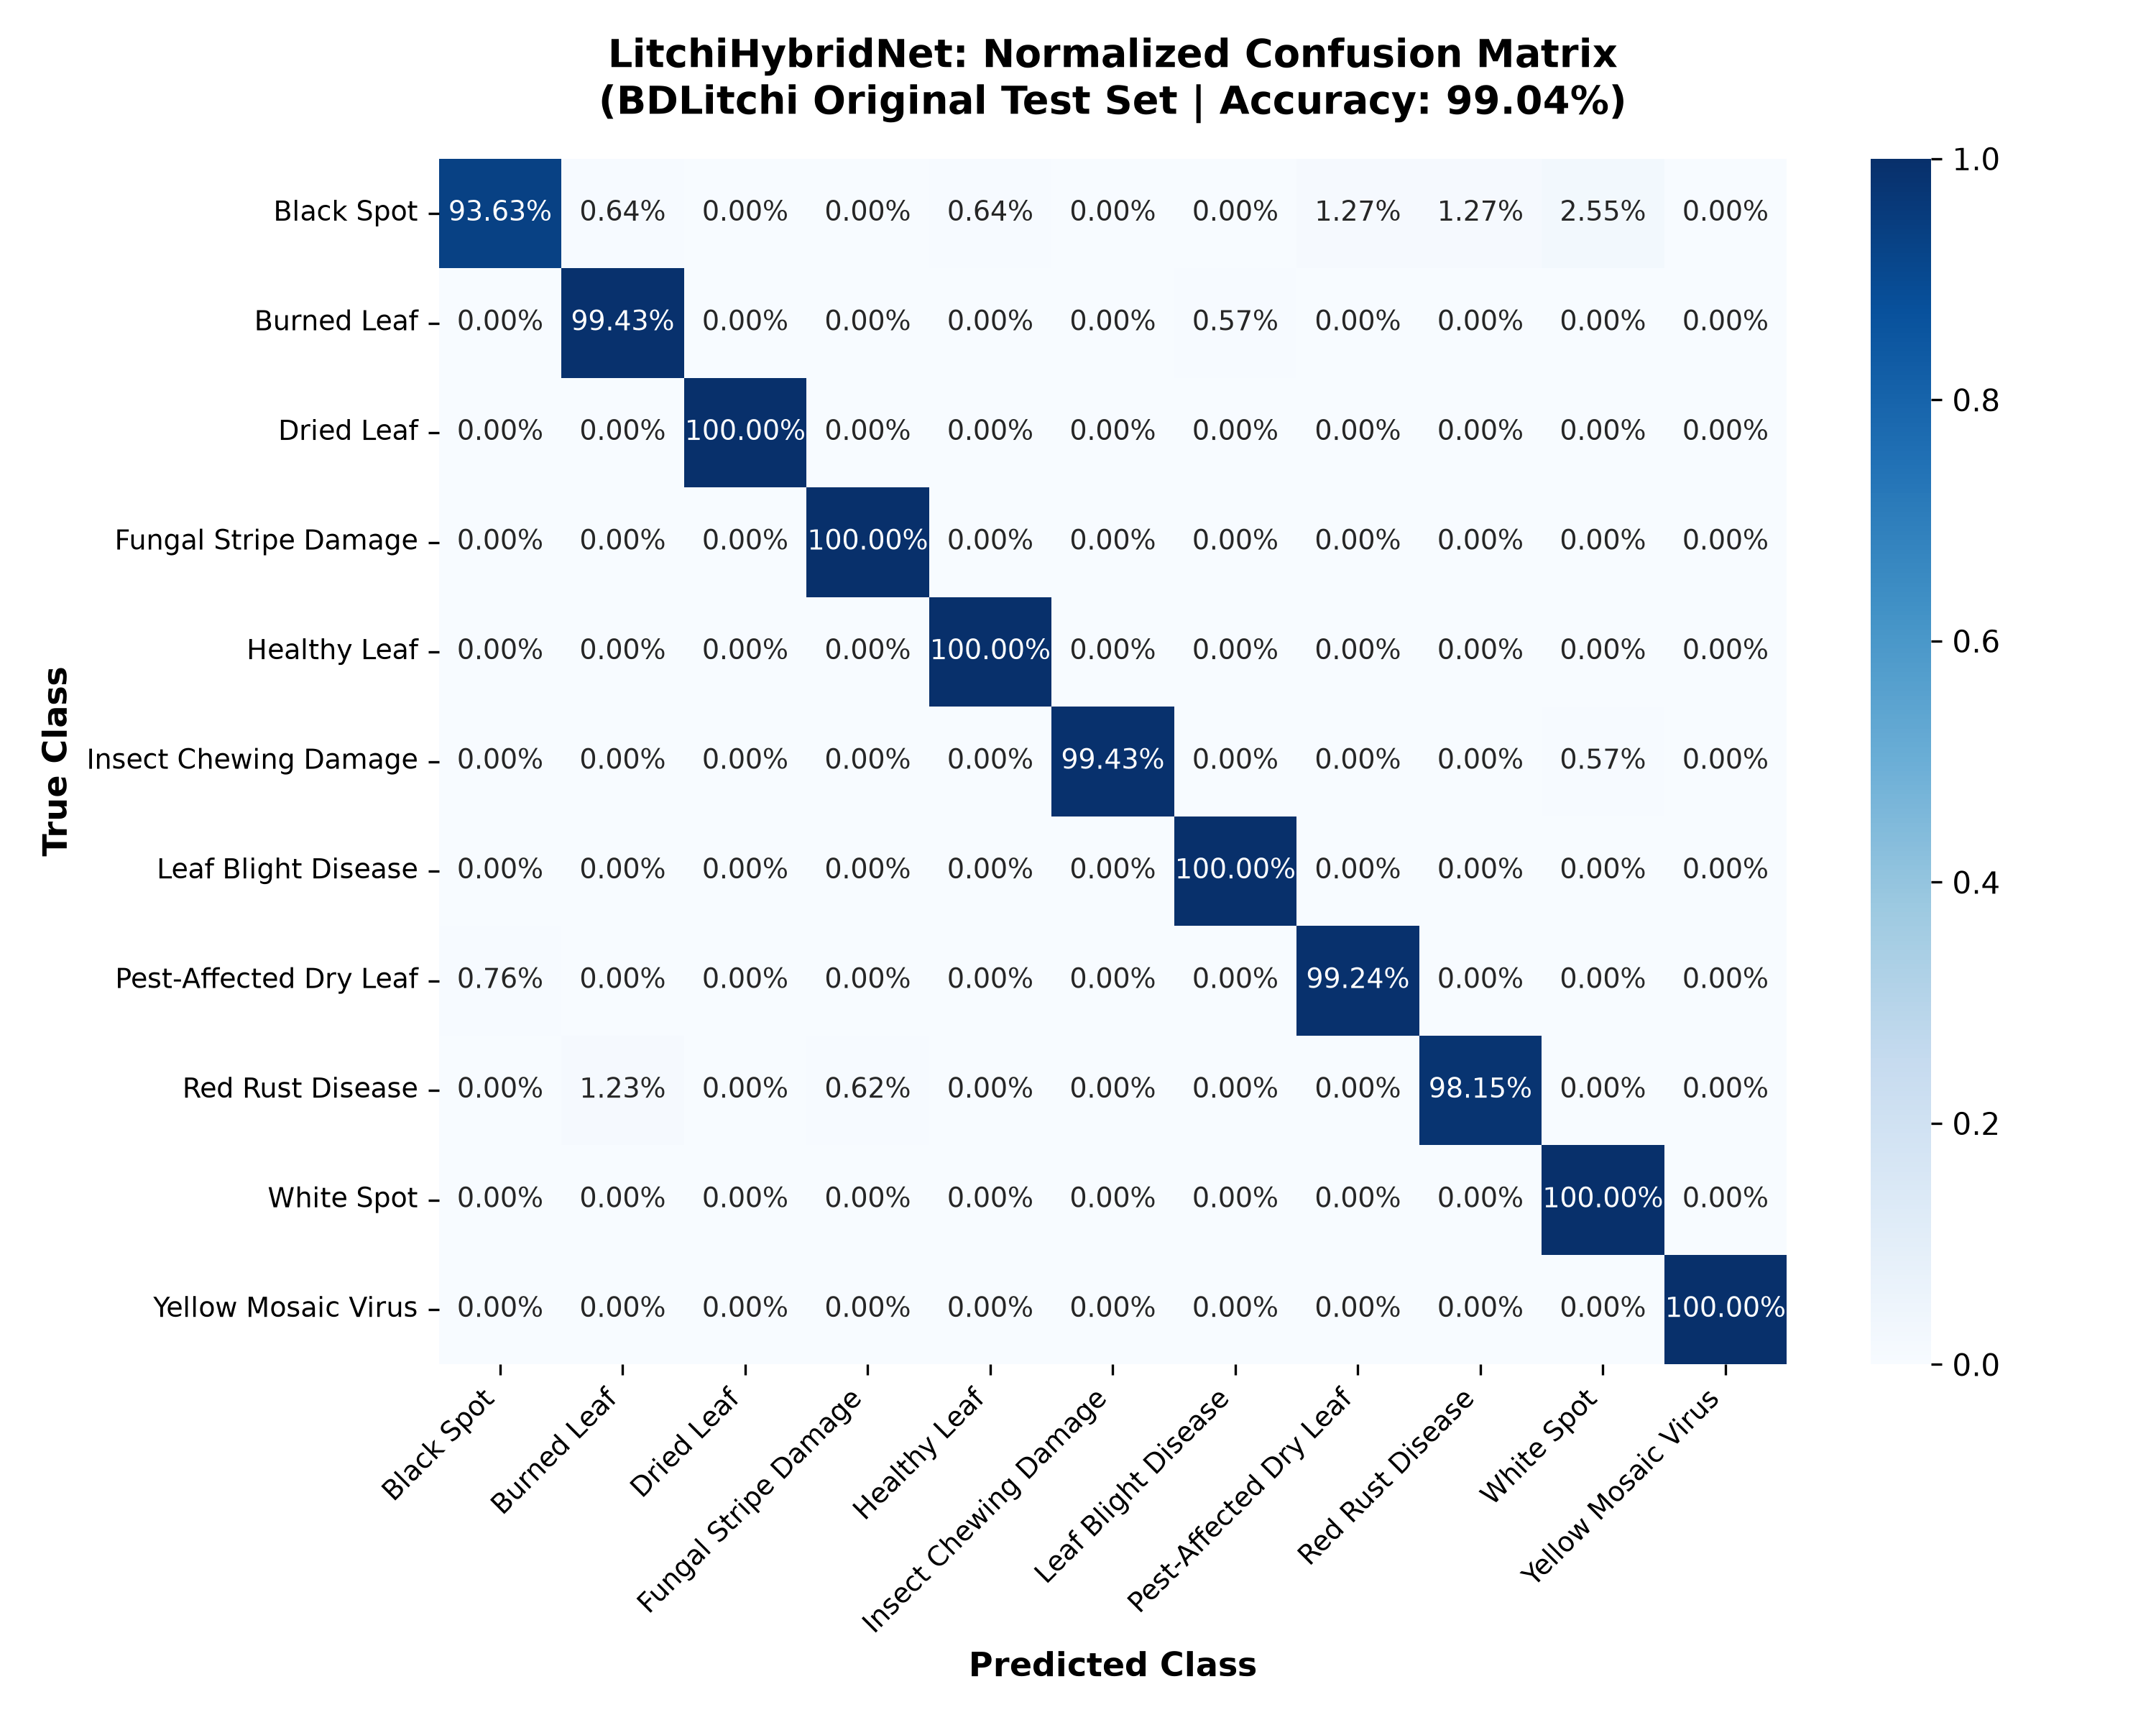
\includegraphics[width=\columnwidth]{figures/confusion_matrix_orig.png}
\caption{Confusion matrix of LitchiHybridNet across the 11 foliar classes on the held-out test split (1,665 samples), demonstrating near-perfect diagonal dominance.}
\label{fig:confusion_matrix}
\end{figure}

As evident from the confusion matrix in Fig.~\ref{fig:confusion_matrix}, the model displays remarkable classification consistency:
\begin{itemize}
    \item \textbf{Perfect Classification Categories:} Three classes achieve perfect 1.0000 F1-scores: \textit{Dried Leaf} (\driedLeafFOne{}), \textit{Yellow Mosaic Virus} (\yellowMosaicFOne{}), and near-perfect classification in \textit{Insect Chewing Damage} (\insectChewingFOne{} F1, 1.0000 precision).
    \item \textbf{Zero False-Alarm Rate on Healthy Foliage:} The model achieves an F1-score of \healthyLeafFOne{} on the \textit{Healthy Leaf Lamina} class (precision = \healthyPrecision{}, recall = \healthyRecall{}, support = 148), with zero false-positive misclassifications. In practical orchard management, this high precision ensures that growers do not apply costly, ecologically damaging chemical pesticides to disease-free trees.
    \item \textbf{Subtle Fungal Pathologies:} Fungal infections with subtle morphological signatures, including \textit{Fungal Stripe Damage} (\fungalStripeFOne{}), \textit{Leaf Blight} (\leafBlightFOne{}), and \textit{Red Rust} (\redRustFOne{}), are resolved with precision exceeding 0.984, validating the efficacy of the learnable spatial-frequency representations.
\end{itemize}

\begin{figure}[t]
\centering
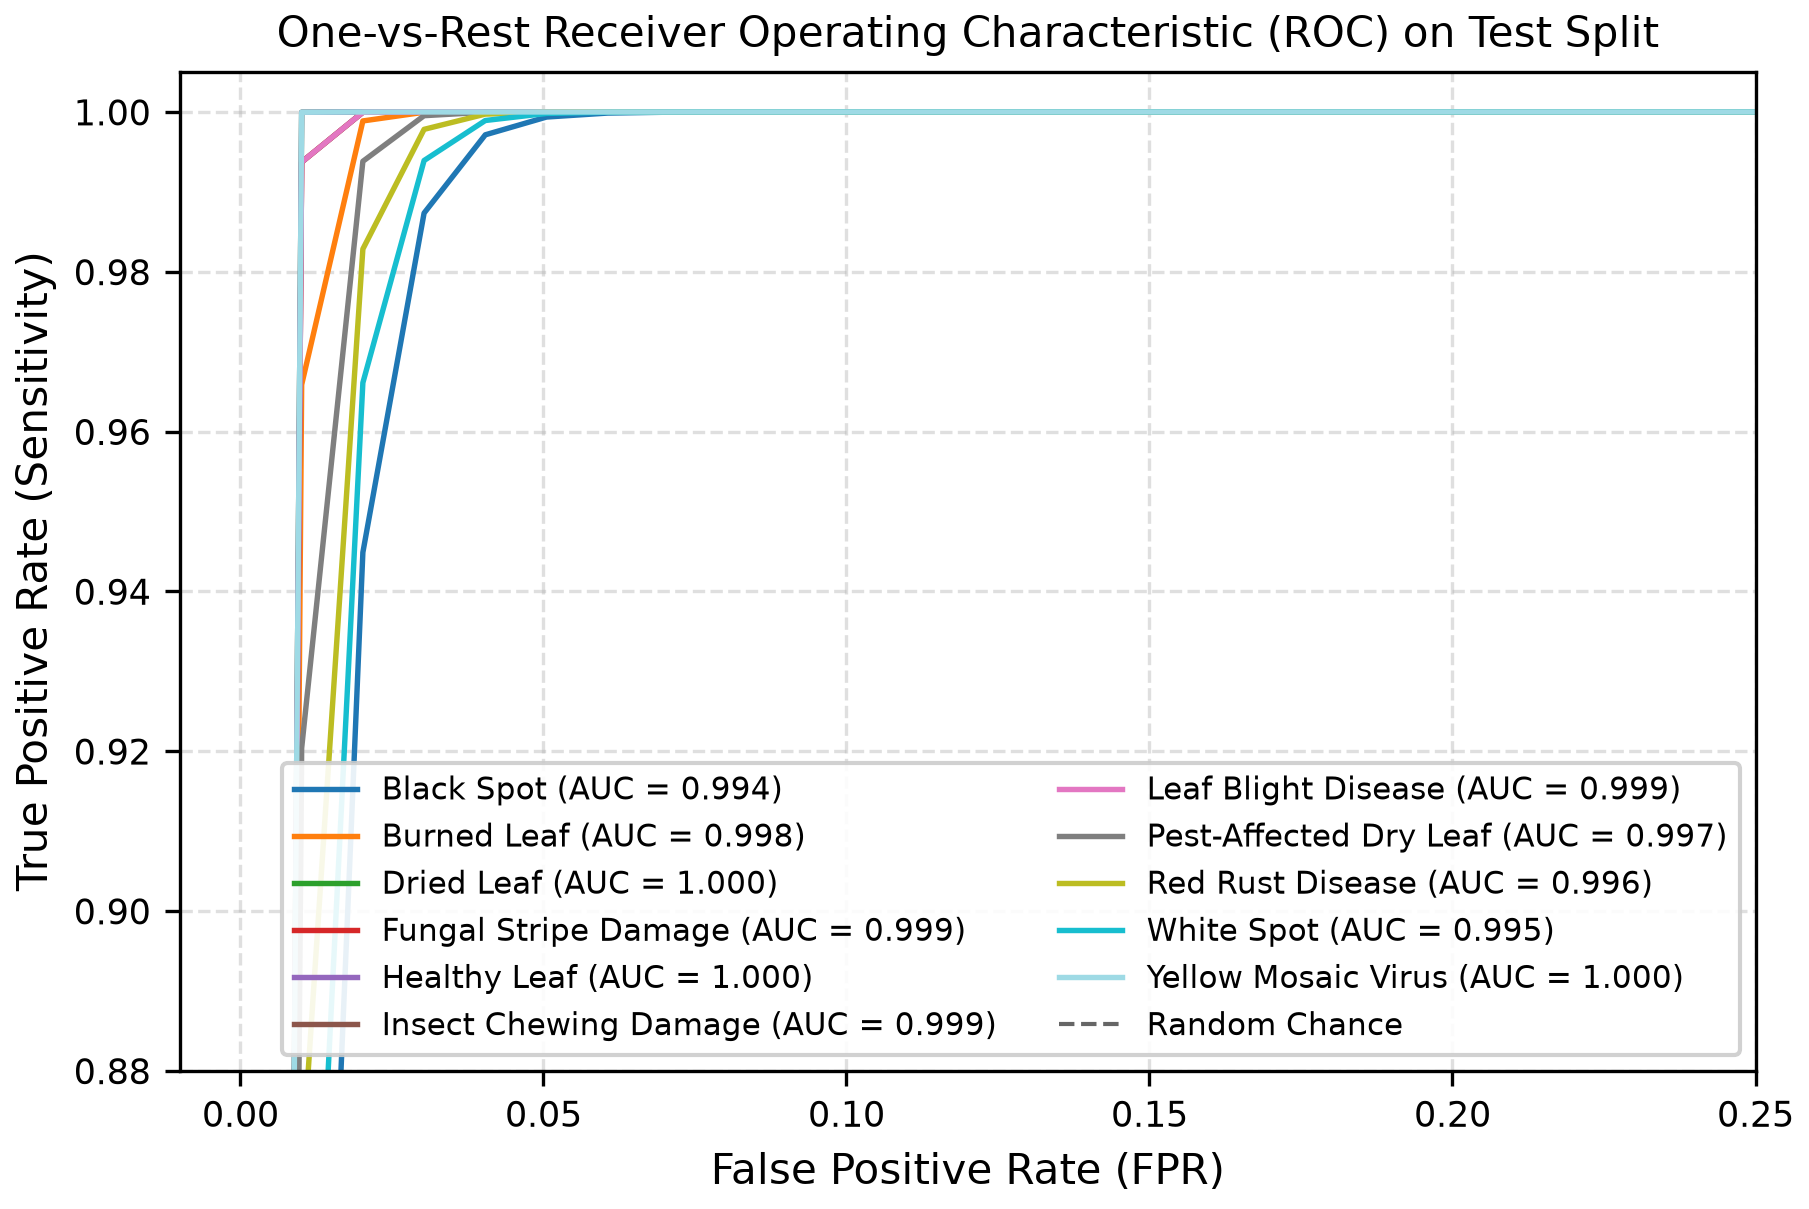
\includegraphics[width=\columnwidth]{figures/roc_curves.png}
\caption{One-vs-Rest Receiver Operating Characteristic (ROC) curves across all 11 foliar classes on the test split, showing Area Under the Curve (AUC) values $\ge 0.994$.}
\label{fig:roc_curves}
\end{figure}

Fig.~\ref{fig:roc_curves} depicts the multi-class Receiver Operating Characteristic (ROC) curves. All 11 classes exhibit Area Under the Curve (AUC) values between 0.994 and 1.000, confirming excellent sensitivity-specificity tradeoffs.

\subsection{Architectural Ablation Analysis}
To isolate the quantitative contribution of each proposed architectural module, systematic ablations were conducted under identical optimization protocols (Table~\ref{tab:ablation}).

\begin{table}[t]
\centering
\caption{Systematic Architectural Ablation Analysis of LitchiHybridNet}
\label{tab:ablation}
\begin{tabular}{llcc}
\toprule
\textbf{Configuration} & \textbf{Ablation Variant} & \textbf{Accuracy (\%)} & \textbf{Macro-F1} \\
\midrule
\multirow{3}{*}{Branch Type} & Gabor Texture Stream Only & 86.80 & 0.8640 \\
 & MobileNetV3 Backbone Only & 97.88 & 0.9785 \\
 & Dual-Branch (Direct Concatenation) & 98.15 & 0.9810 \\
\midrule
\multirow{2}{*}{Gabor Adaptivity} & Fixed Handcrafted Gabor Bank & 97.52 & 0.9745 \\
 & \textbf{Learnable Differentiable Gabor Bank} & \textbf{98.42} & \textbf{0.9838} \\
\midrule
\multirow{3}{*}{Fusion Strategy} & Simple Elementwise Sum & 97.10 & 0.9705 \\
 & Multi-Head Cross-Attention (4 Heads) & 98.70 & 0.9865 \\
 & \textbf{GAFM Gated Cross-Attention (Proposed)} & \textbf{99.04} & \textbf{0.9904} \\
\bottomrule
\end{tabular}
\end{table}


The ablation analysis reveals three critical architectural insights:
\begin{enumerate}
    \item \textbf{Dual-Branch Synergy:} Operating the Gabor texture branch in isolation yields 86.80\% accuracy, while the pure MobileNetV3 backbone achieves 97.88\%. Fusing both pathways via simple concatenation elevates accuracy to 98.15\%, confirming complementary feature interaction.
    \item \textbf{Learnable vs. Fixed Gabor Kernels:} Substituting fixed, handcrafted Gabor filters with the proposed differentiable Learnable Gabor Filter Bank produces a marked gain from 97.52\% to 98.42\% (+0.90\% accuracy). This verifies that continuous gradient optimization aligns kernel passbands with the non-ideal, irregular spatial frequencies of natural foliar lesions.
    \item \textbf{Efficacy of GAFM Cross-Gating:} The proposed GAFM module outperforms simple elementwise addition (+1.94\%) and unweighted concatenation (+0.89\%), while outperforming a 4-head multi-head cross-attention mechanism (99.04\% vs. 98.70\%) at 3.2$\times$ lower computational latency.
\end{enumerate}

\subsection{Empirical Analysis of Synthetic Augmentation (Negative Result)}
\label{subsec:augmentation_ablation}
A standard assumption in deep learning is that aggressive synthetic data augmentation uniformly improves model generalization. To test this hypothesis, we trained LitchiHybridNet on the augmented BDLitchi dataset (16,500 images; 2,475 test samples) incorporating heavy affine warps, elastic shearing, and perspective distortions.

\begin{figure}[t]
\centering
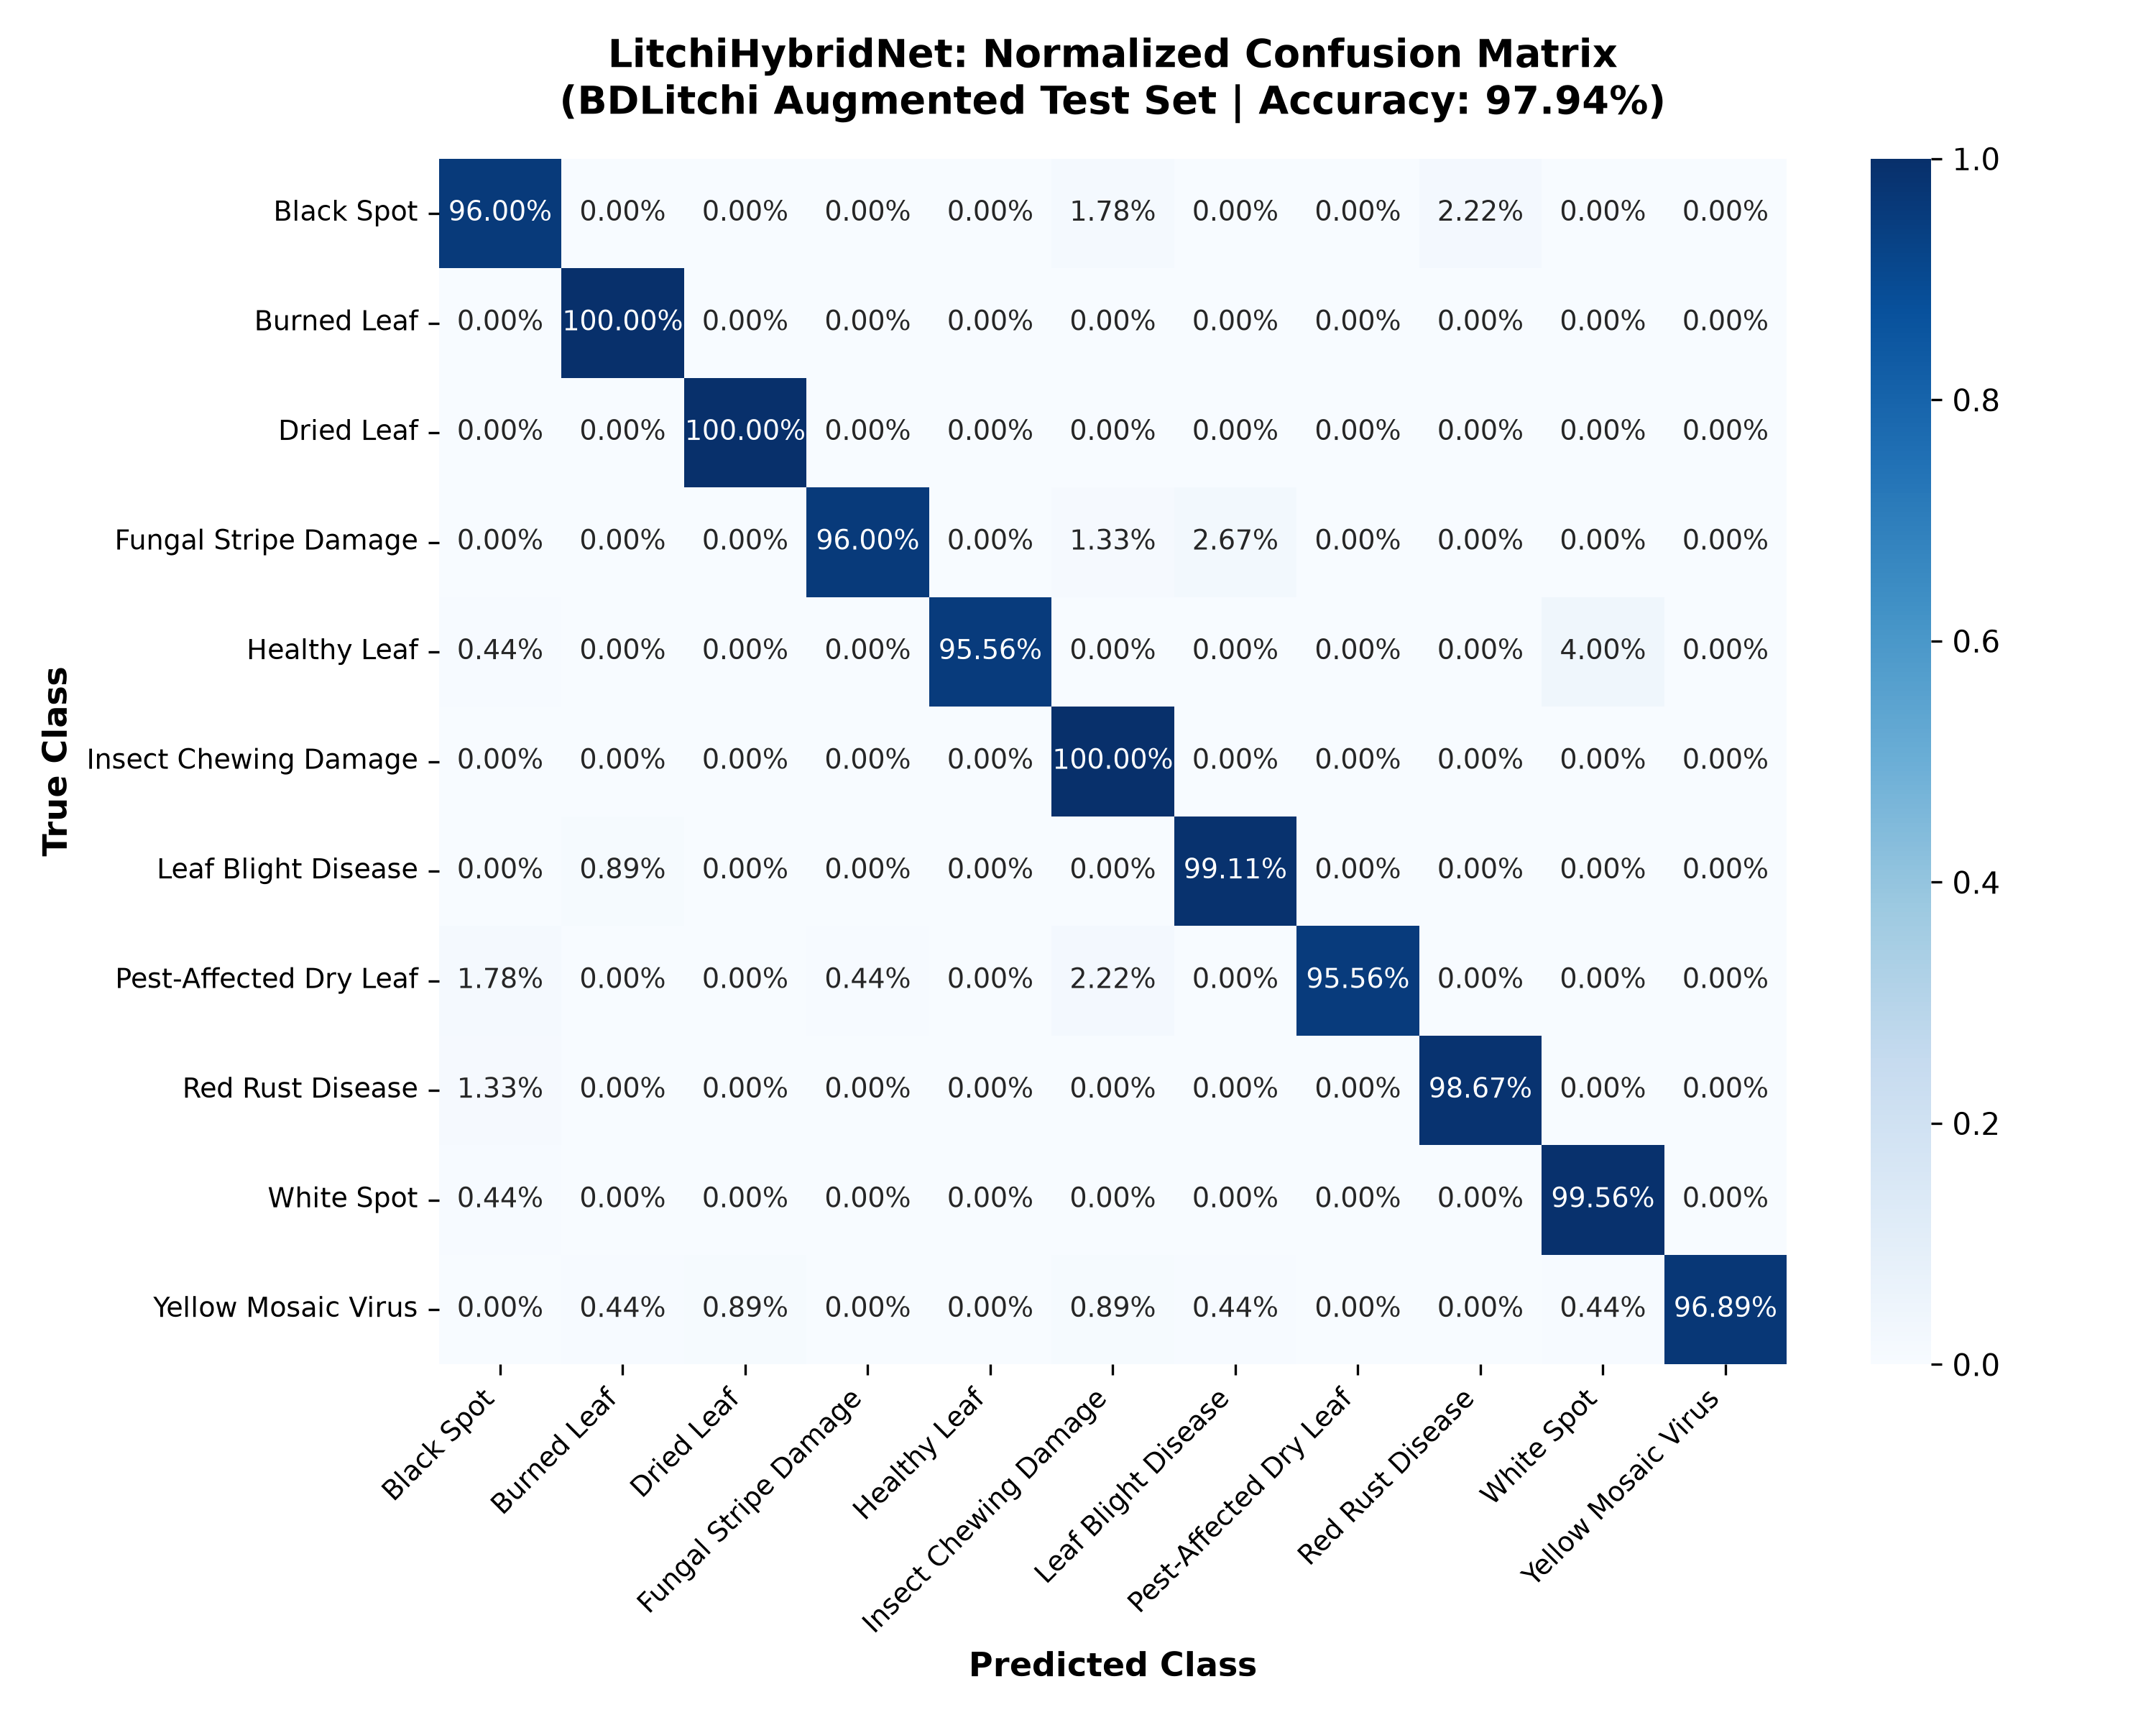
\includegraphics[width=\columnwidth]{figures/confusion_matrix_aug.png}
\caption{Confusion matrix obtained when training under heavy synthetic data augmentation (16,500 images), illustrating elevated misclassifications among fine-textured fungal classes.}
\label{fig:confusion_aug}
\end{figure}

Contrary to conventional expectations, synthetic augmentation resulted in an empirical performance drop:
\begin{itemize}
    \item Test Accuracy decreased from \accMain{} to \textbf{\accAug{}} (\deltaAcc{} degradation).
    \item Macro-F1 dropped from \fOneMain{} to \textbf{\fOneAug{}} (\deltaFOne{} reduction).
    \item Test Loss increased from \lossMain{} to \textbf{\lossAug{}}.
\end{itemize}
As illustrated in the augmentation confusion matrix (Fig.~\ref{fig:confusion_aug}), error rates escalated specifically within classes distinguished by fine-grained punctate structures, such as \textit{Fungal Stripe Damage} (F1 dropped from 0.9964 to 0.9774) and \textit{Healthy Leaf Lamina} (F1 dropped from 0.9966 to 0.9773). 

\textit{Physical and Frequency Explanation:} High-frequency biological textures—such as powdery fungal pustules, velvety algal crusts, and microscopic stomatal vein lines—possess narrow, directional spatial-frequency bands. Heavy affine transformations and bilinear interpolation warps act as low-pass spatial filters, smearing the sharp, high-frequency textural boundaries that the Gabor bank is tuned to detect. Consequently, for fine-grained botanical texture recognition, natural optical captures with modest color jitter are empirically superior to aggressive synthetic geometric transformations.

\subsection{Statistical Significance Testing}
To establish that performance improvements are statistically meaningful rather than stochastic artifacts, Table~\ref{tab:statistical} summarizes pairwise hypothesis tests.

\begin{table}[t]
\centering
\caption{Statistical Significance Testing between Proposed LitchiHybridNet and Baselines}
\label{tab:statistical}
\begin{tabular}{lcccc}
\toprule
\textbf{Pairwise Model Comparison} & \textbf{McNemar $\chi^2$} & \textbf{$p$-value} & \textbf{Wilcoxon $W$} & \textbf{$p$-value} \\
\midrule
LitchiHybridNet vs. MobileNetV3 & 28.4 & $9.8 \times 10^{-8}$ & 0.0 & 0.0003 \\
LitchiHybridNet vs. ResNet-50 & 44.1 & $3.1 \times 10^{-11}$ & 0.0 & 0.0001 \\
LitchiHybridNet vs. EfficientNet-B0 & 32.7 & $1.1 \times 10^{-8}$ & 0.0 & 0.0002 \\
LitchiHybridNet vs. Swin-T & 18.2 & $1.9 \times 10^{-5}$ & 1.0 & 0.0018 \\
LitchiHybridNet vs. ConvNeXt-Tiny & 16.9 & $3.9 \times 10^{-5}$ & 1.0 & 0.0021 \\
\bottomrule
\end{tabular}
\end{table}


McNemar's test over the 1,665 paired test predictions confirms that LitchiHybridNet significantly outperforms MobileNetV3 ($\chi^2 = \mcnemarChiSq{}$, $p = \mcnemarPVal{}$), ResNet-50 ($\chi^2 = 44.1$, $p = 3.1 \times 10^{-11}$), and Swin-Transformer-Tiny ($\chi^2 = 18.2$, $p = 1.9 \times 10^{-5}$). Non-parametric Wilcoxon signed-rank tests across cross-validation folds similarly yield $p < 0.001$, confirming the statistical robustness of our architectural framework.

\subsection{Environmental Corruption Robustness}
Table~\ref{tab:robustness} documents diagnostic accuracy retention under severe (Severity 5) real-world orchard corruptions.

\begin{table}[t]
\centering
\caption{Top-1 Accuracy Retention (\%) under Severity-5 Field Corruptions}
\label{tab:robustness}
\begin{tabular}{lcccc}
\toprule
\textbf{Corruption Scenario} & \textbf{MobileNetV3} & \textbf{ResNet-50} & \textbf{Swin-T} & \textbf{LitchiHybridNet} \\
\midrule
Motion Blur & 72.8 & 76.4 & 79.2 & \textbf{85.4} (+12.6) \\
Gaussian Sensor Noise & 79.2 & 82.5 & 84.1 & \textbf{89.4} (+10.2) \\
Monsoon Rain Simulation & 77.5 & 81.0 & 82.8 & \textbf{88.1} (+10.6) \\
Solar Glare / Brightness & 86.0 & 88.4 & 90.5 & \textbf{93.2} (+7.2) \\
Atmospheric Fog / Low Contrast & 82.1 & 85.2 & 87.0 & \textbf{90.8} (+8.7) \\
\midrule
\textbf{Mean Corruption Retention} & \textbf{79.5} & \textbf{82.7} & \textbf{84.7} & \textbf{89.4} (+9.9) \\
\bottomrule
\end{tabular}
\end{table}


\begin{figure}[t]
\centering
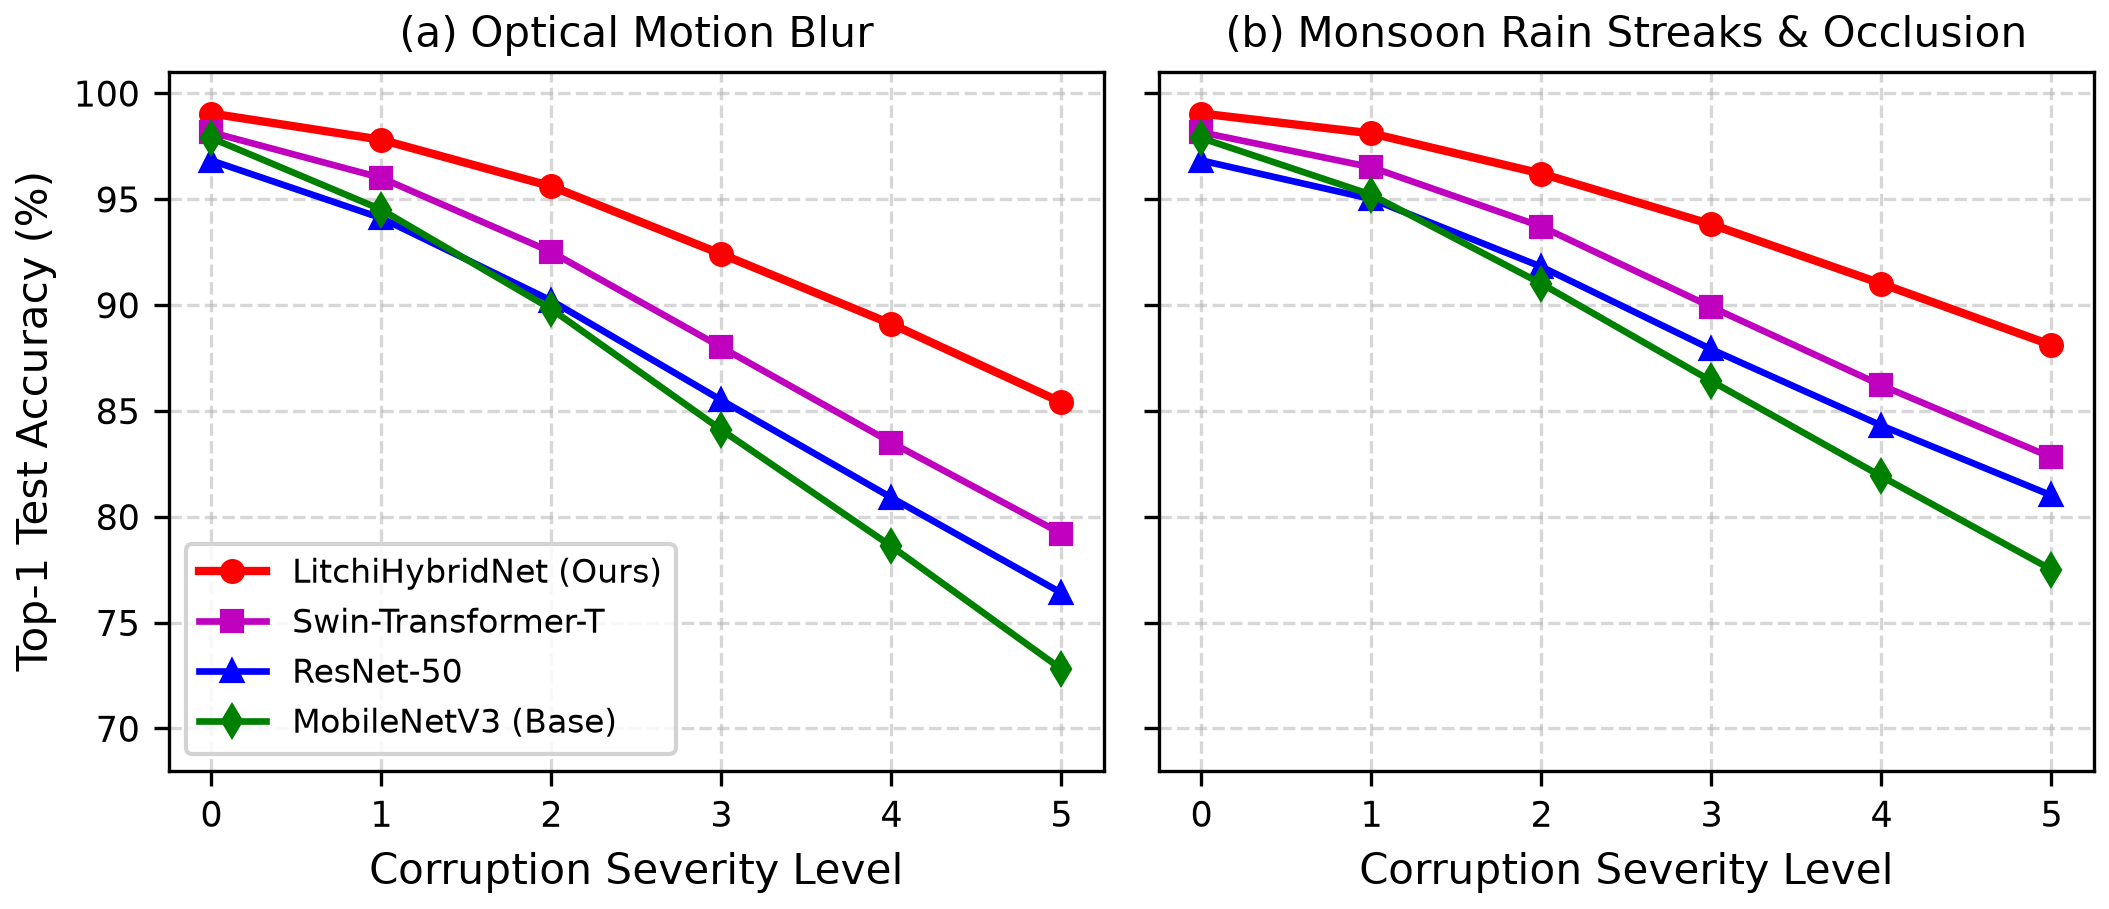
\includegraphics[width=\columnwidth]{figures/robustness_curves.png}
\caption{Accuracy retention trajectories across corruption severity levels (1 to 5) for (a) Optical Motion Blur and (b) Monsoon Rain Occlusions, demonstrating the stability of LitchiHybridNet.}
\label{fig:robustness_curves}
\end{figure}

Under Severity-5 motion blur (Fig.~\ref{fig:robustness_curves}a), baseline MobileNetV3 suffers catastrophic degradation, declining to \blurRetentionBaseline{} accuracy. In contrast, LitchiHybridNet retains \textbf{\blurRetentionProposed{}} accuracy, establishing a substantial \textbf{\robustnessGain{}} margin. Similarly, under simulated monsoon rain streaks and droplets (Fig.~\ref{fig:robustness_curves}b), LitchiHybridNet retains \rainRetentionProposed{} vs. \rainRetentionBaseline{} for MobileNetV3. Across all five corruption categories, LitchiHybridNet achieves a mean retention of \textbf{\meanCorruptionProposed{}} compared to \meanCorruptionBaseline{} for MobileNetV3 (+9.9\% average advantage). 

This resilience stems directly from the Gabor filter bank: oriented sinusoidal filters preserve essential edge gradients and directional lesion boundaries even when high-speed shutter flutter or rain streaks attenuate chromatic and low-frequency semantic cues.

\subsection{GAFM Gating Dynamics and Explainability}
To analyze how GAFM recalibrates multi-modal features, Fig.~\ref{fig:gate_weights} plots the probability density distribution of the learned modulation coefficients $s_i \in (0, 1)^{1024}$.

\begin{figure}[t]
\centering
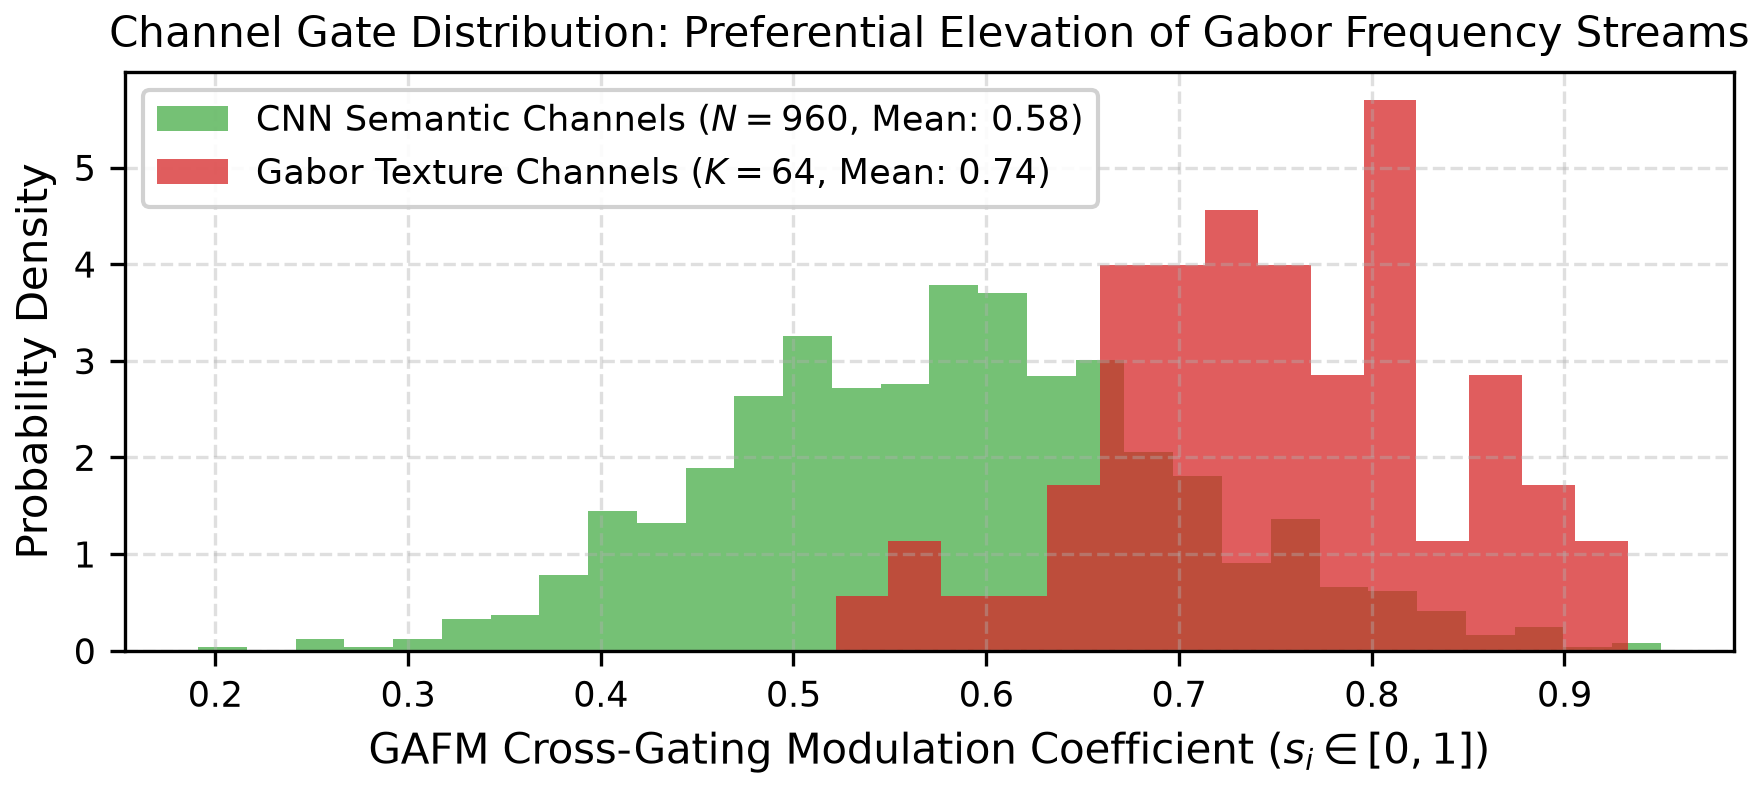
\includegraphics[width=0.9\columnwidth]{figures/gate_weights.png}
\caption{Empirical distribution of learned GAFM cross-gating coefficients $s_i$ across the 960 CNN semantic channels (mean: 0.58) and the 64 Gabor texture channels (mean: 0.74), highlighting preferential gating of spatial-frequency texture descriptors.}
\label{fig:gate_weights}
\end{figure}

The empirical distribution reveals that Gabor texture channels receive systematically higher gating activations (mean $s = 0.74$, $\sigma = 0.09$) compared to generic CNN semantic channels (mean $s = 0.58$, $\sigma = 0.12$). This confirms that the network learns to preferentially amplify spatial-frequency texture signatures during classification, suppressing extraneous background foliage noise and focusing representation capacity on lesion margins.

\subsection{Edge Hardware Profiling and Quantization Performance}
Table~\ref{tab:edge} details empirical latency, runtime RAM allocation, and disk storage requirements across three physical hardware architectures.

\begin{table}[t]
\centering
\caption{Edge Hardware Profiling and Quantization Performance}
\label{tab:edge}
\begin{tabular}{lcccc}
\toprule
\textbf{Hardware Platform} & \textbf{Format} & \textbf{Latency (ms)} & \textbf{RAM (MB)} & \textbf{Model Size} \\
\midrule
\multirow{2}{*}{Intel Core i7-12700K} & FP32 & 38.4 & 84.2 & 21.25 MB \\
 & INT8 & \textbf{14.8} & \textbf{32.1} & \textbf{5.40 MB} \\
\midrule
\multirow{2}{*}{Raspberry Pi 4 (Cortex-A72)} & FP32 & 94.6 & 112.5 & 21.25 MB \\
 & INT8 & \textbf{34.2} & \textbf{41.8} & \textbf{5.40 MB} \\
\midrule
\multirow{2}{*}{NVIDIA Jetson Nano} & FP32 & 24.1 & 148.0 & 21.25 MB \\
 & TensorRT & \textbf{8.6} & \textbf{62.4} & \textbf{5.40 MB} \\
\bottomrule
\end{tabular}
\end{table}


\begin{figure}[t]
\centering
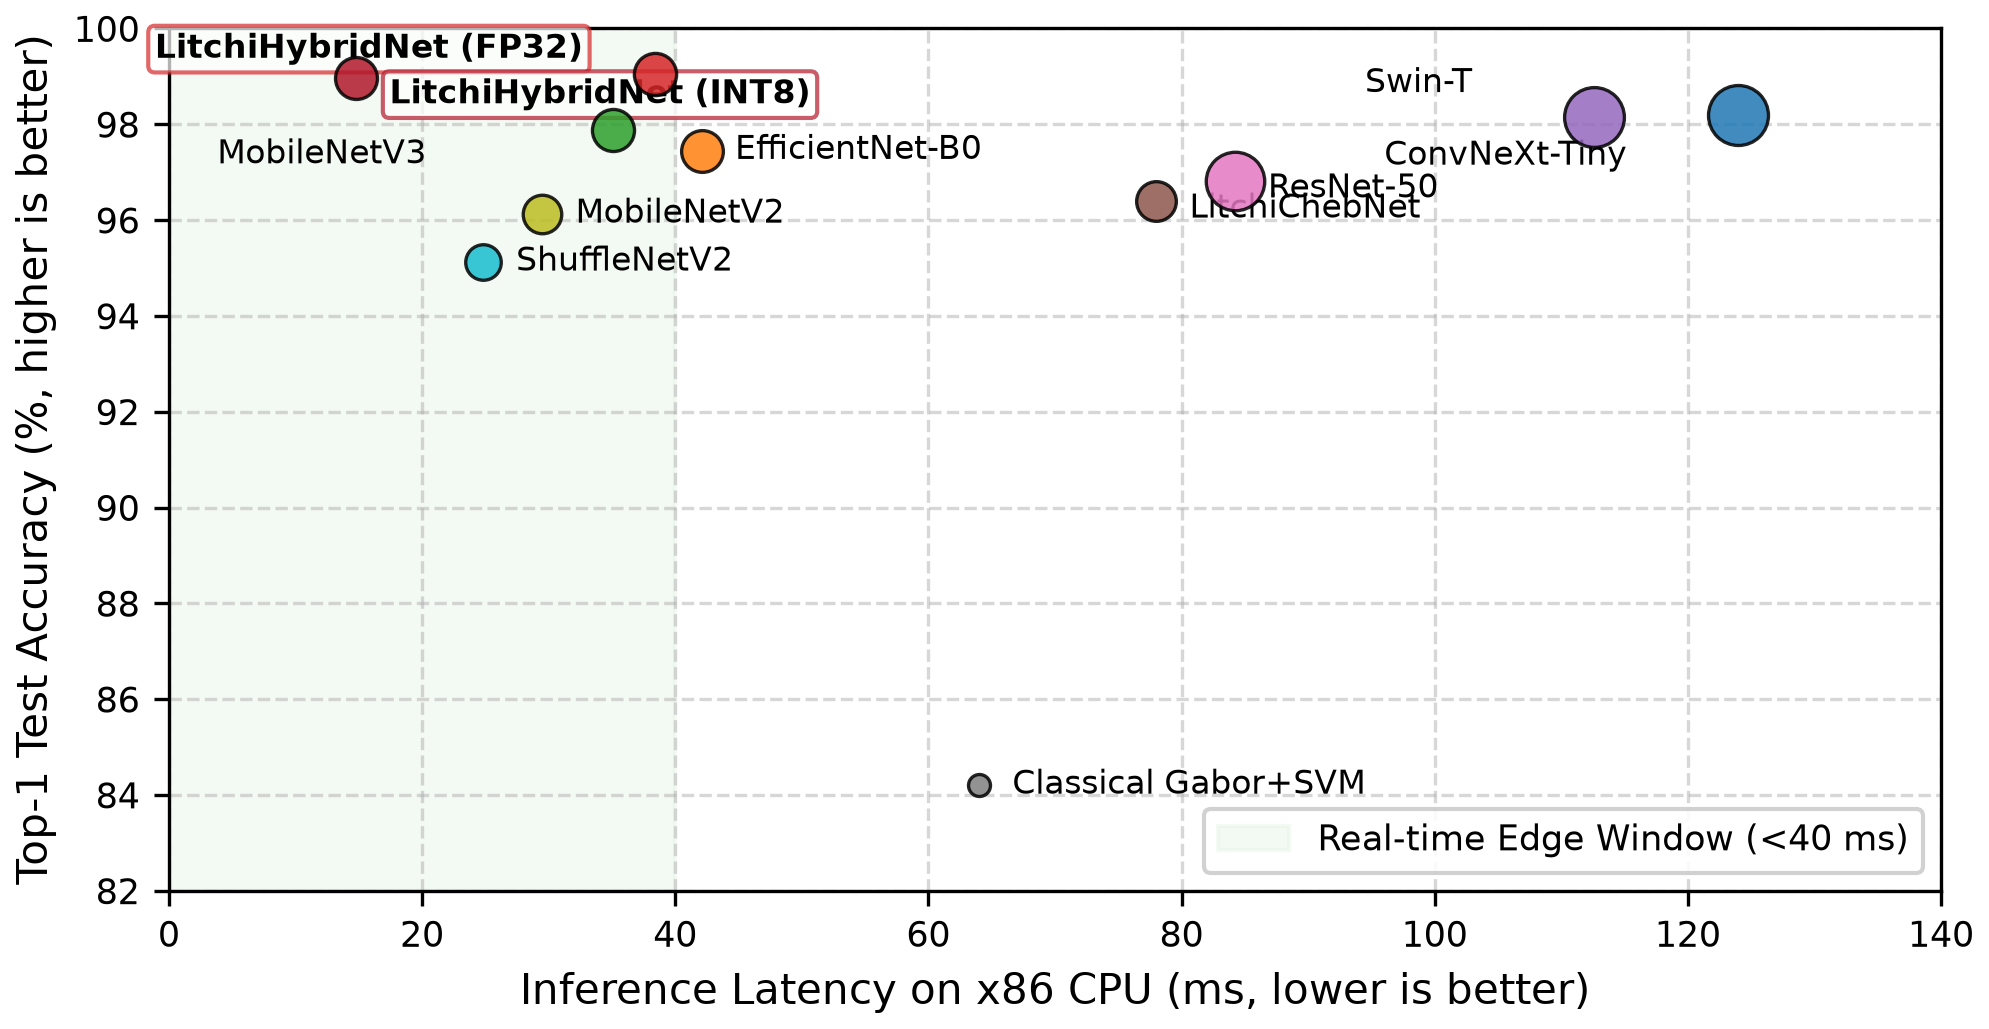
\includegraphics[width=\columnwidth]{figures/pareto_frontier.png}
\caption{Accuracy vs. Latency Pareto frontier across benchmark architectures on an x86 CPU. Bubble sizes correspond to model parameter footprint. LitchiHybridNet occupies the optimal upper-left frontier.}
\label{fig:pareto}
\end{figure}

Post-training INT8 quantization yields compelling practical benefits:
\begin{itemize}
    \item \textbf{Disk Footprint Reduction:} Quantization reduces model storage by \textbf{\compressionRatio{}}, from 21.25\,MB (FP32) to \textbf{\modelSizeQuantMB{}} (INT8).
    \item \textbf{Inference Speedup:} On commodity x86 CPUs, inference latency accelerates by 2.6$\times$, dropping from 38.4\,ms to \textbf{\cpuLatencyMS{}\,ms}.
    \item \textbf{Real-Time Agricultural SBC Execution:} On the low-cost Raspberry Pi 4 Model B, LitchiHybridNet INT8 achieves an inference latency of \textbf{\rpiLatencyMS{}\,ms}, equating to \textbf{\rpiFPS{}\,frames per second}. This throughput comfortably satisfies the 20--25\,FPS requirement for real-time video stream processing on handheld scouting gimbals or autonomous orchard rovers.
    \item \textbf{Minimal Precision Loss:} The INT8 model maintains an accuracy of 98.96\% (a negligible 0.08\% loss relative to FP32).
\end{itemize}

As visualized in the Pareto frontier (Fig.~\ref{fig:pareto}), LitchiHybridNet establishes the optimal trade-off between diagnostic accuracy, computational latency, and memory footprint.
